\newpage
\section{LATEX}
\indent Para entender o que é LaTeX é necessário conhecer o TeX, um programa criado pelo renomado cientista da computação, Donald Knuth, na década de 70. O TeX foi criado com o objetivo de aumentar a qualidade impressa de textos, especialmente para textos que apresentassem caracteres matemáticos \cite{oetiker2001}.

Já o LaTeX, foi criado na década de 80 por Leslie Lamport. Ele é um programa que reúne uma coleção de comandos que utilizam o TeX como base de processamento. Ele possui distribuição para os principais sistemas operacionais: Windows, Linux e Macosx \cite{oetiker2001}.

Dentre suas principais vantagens pode-se citar:

•	Controle sobre documentos grandes contendo seções, tabelas, figuras, etc.

•	Tipografia de fórmulas matemáticas complexas.

•	Geração automática de bibliografias e índices.

•	Está disponível como software livre.\\

\subsection{INSTALAÇÃO}
Para utilizar o LaTeX é necessário a instalação do MiKTeX, uma implementação atualizada do LaTeX \cite{miktex2018}, e um editor de LaTeX.

O MikTeX vem com o TeXworks pré-instalado, porém existem editores mais completos, como o TeXMaker, o TeXstudio e o TeXnicCenter. O TeXMaker foi escolhido, pois é um editor LaTeX gratuito, moderno e multiplataforma para sistemas Linux, Macosx e Windows e pela sua facilidade de uso e configuração \cite{texmaker2018}.

Os passos relatados a seguir referem-se à instalação no sistema operacional Windows, nas versões 7, 8 e 10 (64-bit).

\newpage
\subsubsection{Instalação do MikTeX}
Para instalar o MiKTeX é necessário acessar o link: https://miktex.org/download e clicar no botão download para realizar o download.

\begin{figure}[htb]
  \begin{center}
    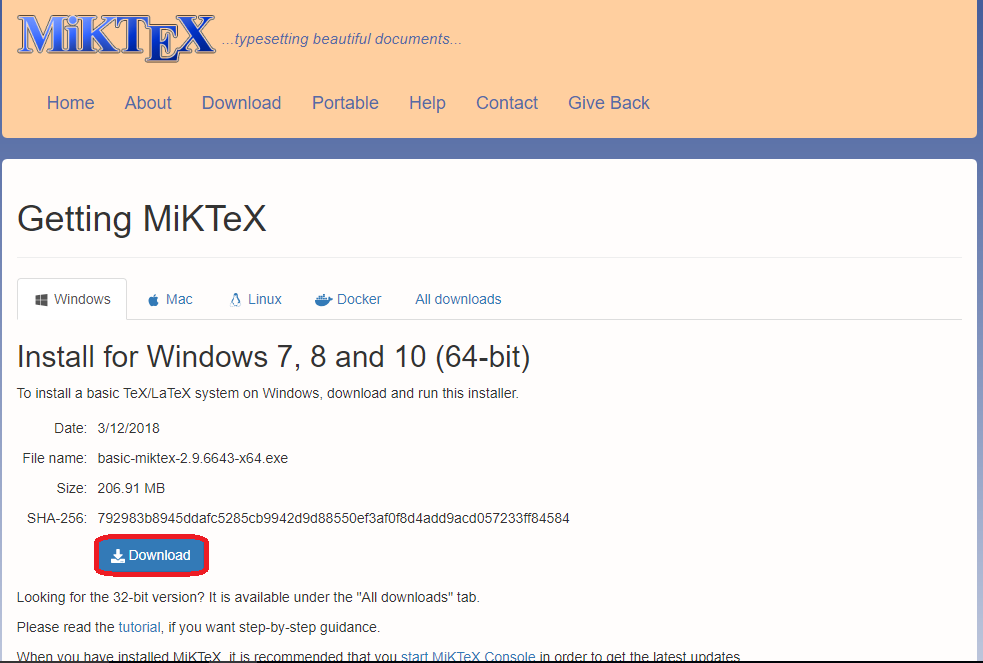
\includegraphics[scale=0.4]{imagens/miktex/miktex1.png}
  \end{center}
  \caption{Instalação do MikTeX - Passo 1.}
  \label{mt1}
\end{figure}

Abra o arquivo de instalação do MiKTeX.\\

\begin{figure}[htb]
  \begin{center}
    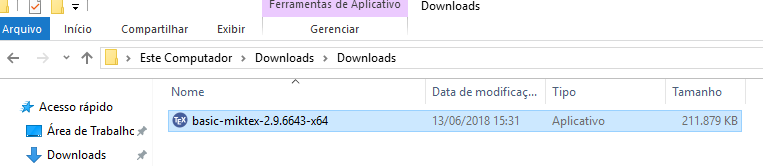
\includegraphics[scale=0.6]{imagens/miktex/miktex2.png}
  \end{center}
  \caption{Instalação do MikTeX - Passo 2.}
  \label{mt2}
\end{figure}

\newpage
Clique em “I accept the MiKTeX copying conditions” e depois em “Avançar$>$”.\\

\begin{figure}[htb]
  \begin{center}
    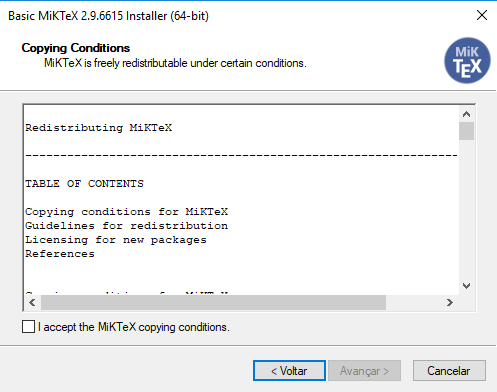
\includegraphics[scale=0.7]{imagens/miktex/miktex3.png}
  \end{center}
  \caption{Instalação do MikTeX - Passo 3.}
  \label{mt3}
\end{figure}

Escolha para quais usuários quer instalar o MiKTeX e clique em “Avançar$>$”.\\

\begin{figure}[htb]
  \begin{center}
    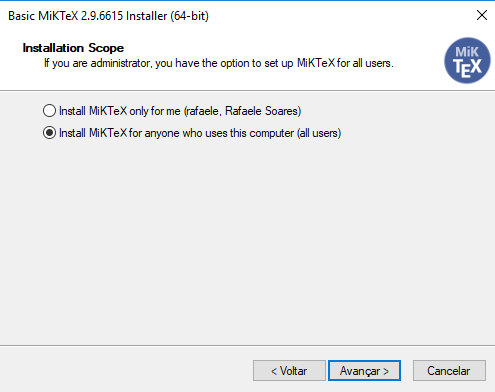
\includegraphics[scale=0.7]{imagens/miktex/miktex4.png}
  \end{center}
  \caption{Instalação do MikTeX - Passo 4.}
  \label{mt4}
\end{figure}

\newpage
Escolha o diretório de instalação e clique em “Avançar$>$”.\\

\begin{figure}[htb]
  \begin{center}
    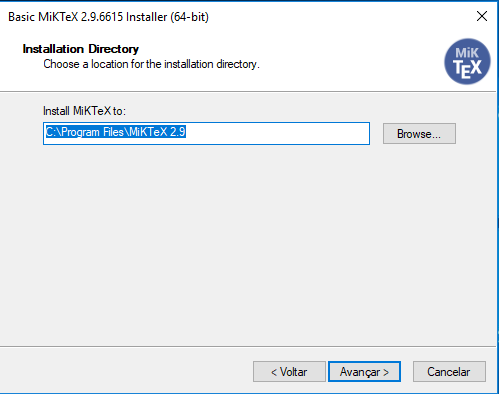
\includegraphics[scale=0.7]{imagens/miktex/miktex5.png}
  \end{center}
  \caption{Instalação do MikTeX - Passo 5 .}
  \label{mt5}
\end{figure}

Configure suas preferências clique em “Avançar$>$”.\\

\begin{figure}[htb]
  \begin{center}
    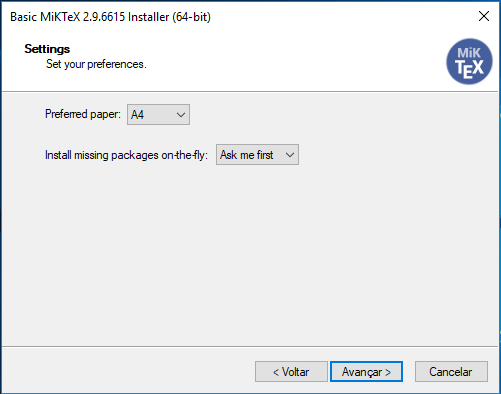
\includegraphics[scale=0.7]{imagens/miktex/miktex6.png}
  \end{center}
  \caption{Instalação do MikTeX - Passo 6.}
  \label{mt6}
\end{figure}

\newpage
Clique em “Start” para iniciar o processo de instalação.\\

\begin{figure}[htb]
  \begin{center}
    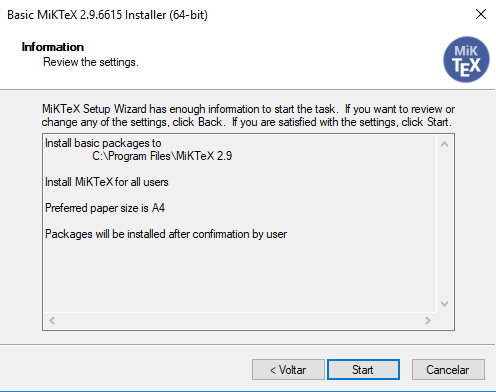
\includegraphics[scale=0.7]{imagens/miktex/miktex7.png}
  \end{center}
  \caption{Instalação do MikTeX - Passo 7.}
  \label{mt7}
\end{figure}

Aguarde a instalação terminar e clique em “Avançar$>$”.\\

\begin{figure}[htb]
  \begin{center}
    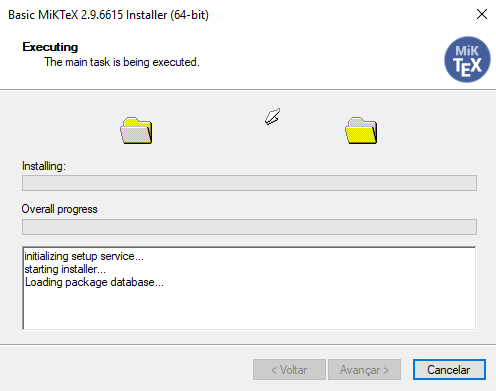
\includegraphics[scale=0.7]{imagens/miktex/miktex8.png}
  \end{center}
  \caption{Instalação do MikTeX - Passo 8.}
  \label{mt8}
\end{figure}

\newpage
Clique em “Close” para fechar a instalação.

\begin{figure}[htb]
  \begin{center}
    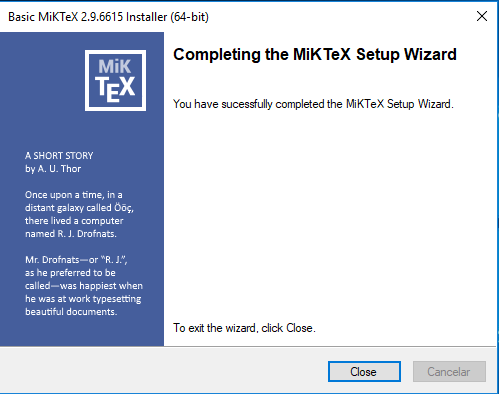
\includegraphics[scale=0.7]{imagens/miktex/miktex9.png}
  \end{center}
  \caption{Instalação do MikTeX - Passo 9.}
  \label{mt9}
\end{figure}

\subsubsection{Instalação do TeXMaker}
Para instalar o TexMaker é necessário acessar o link:

http://www.xm1math.net/texmaker/download.html e clicar na versão que deseja realizar o download.\\

\begin{figure}[htb]
  \begin{center}
    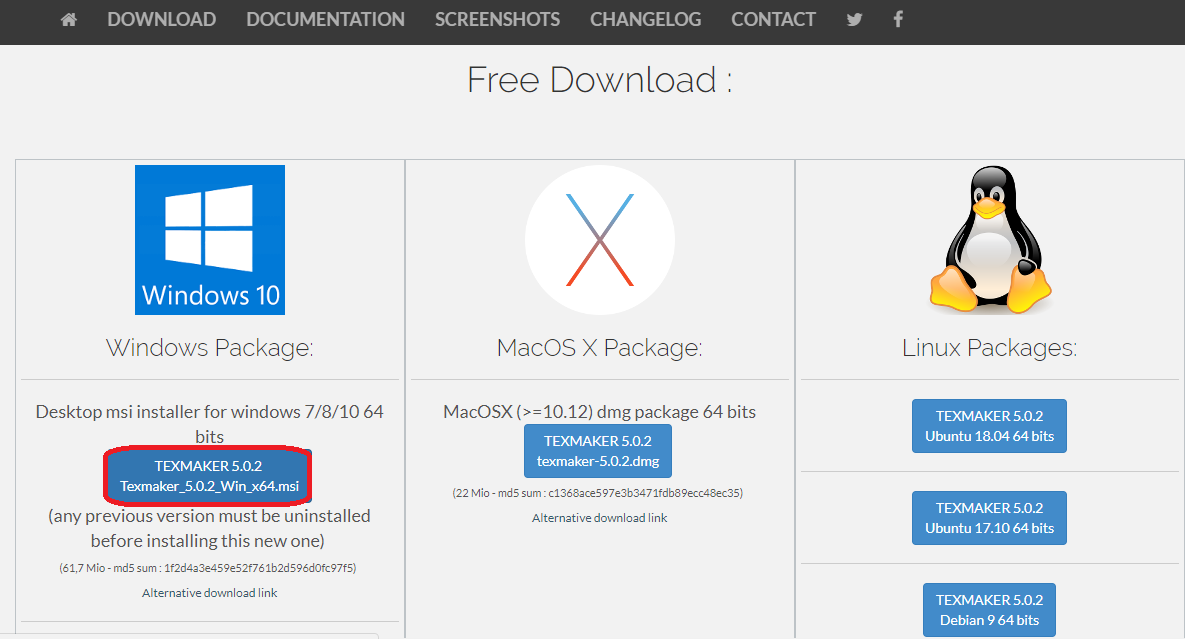
\includegraphics[scale=0.35]{imagens/texmaker/texmaker1.png}
  \end{center}
  \caption{Instalação do TeXMaker - Passo 1.}
  \label{tmk1}
\end{figure}

\newpage
Abra o arquivo de instalação do TexMaker.

\begin{figure}[htb]
  \begin{center}
    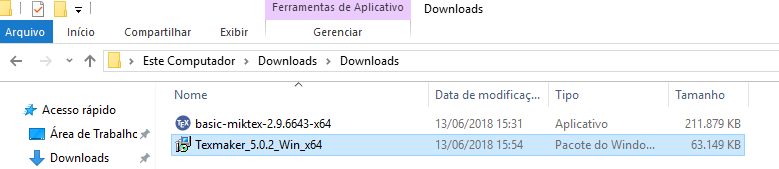
\includegraphics[scale=0.5]{imagens/texmaker/texmaker2.png}
  \end{center}
  \caption{Instalação do TeXMaker - Passo 2.}
  \label{tmk2}
\end{figure}

Clique em “I accept the terms in the license Agreement” e depois em “Install”.

\begin{figure}[htb]
  \begin{center}
    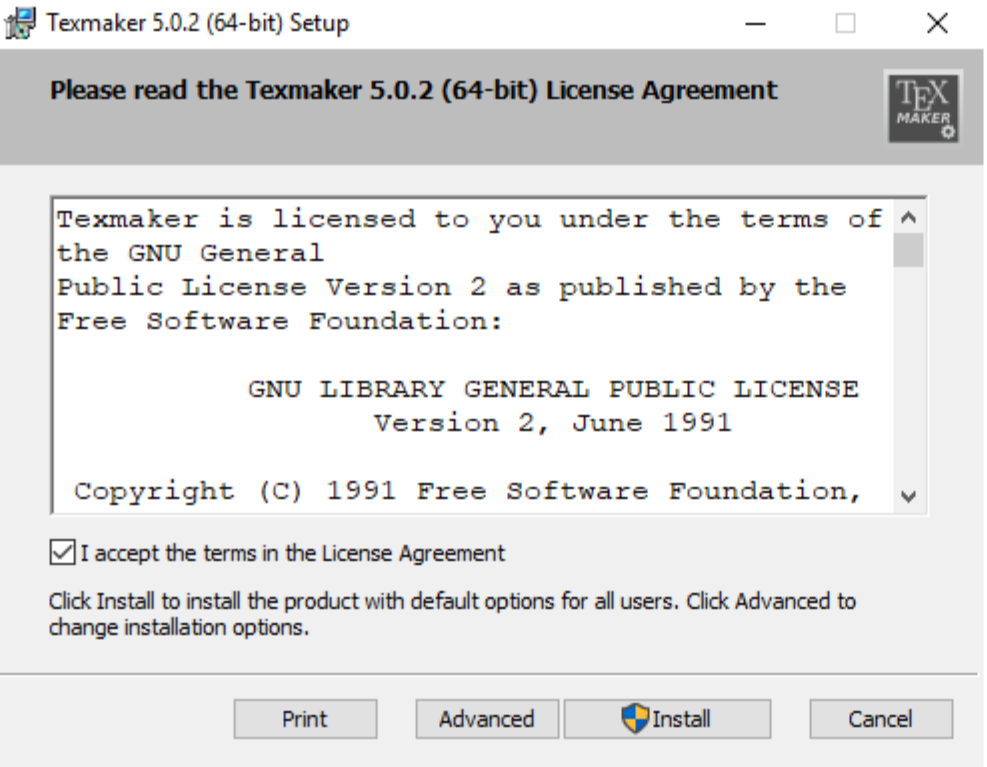
\includegraphics[scale=0.3]{imagens/texmaker/texmaker3.png}
  \end{center}
  \caption{Instalação do TeXMaker - Passo 3.}
  \label{tmk3}
\end{figure}

Aguarde a instalação terminar e clique em “Next”.

\begin{figure}[h!]
  \begin{center}
    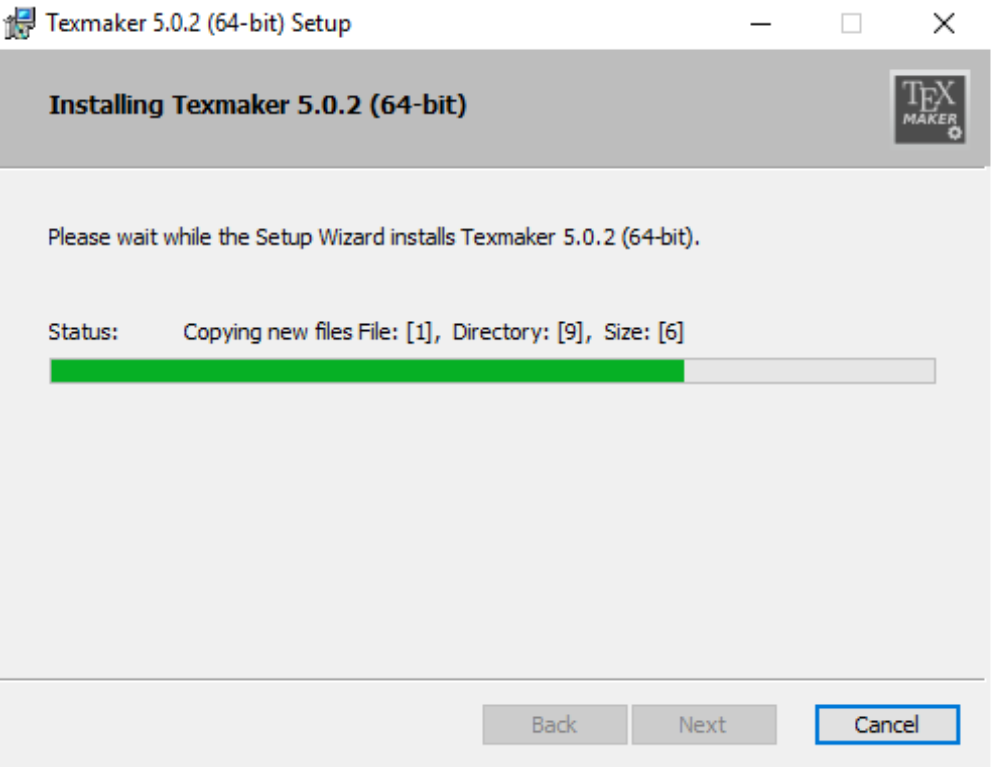
\includegraphics[scale=0.3]{imagens/texmaker/texmaker4.png}
  \end{center}
  \caption{Instalação do TeXMaker - Passo 4.}
  \label{tmk4}
\end{figure}

\newpage
Clique em “Finish” para fechar a instalação.

\begin{figure}[h!]
  \begin{center}
    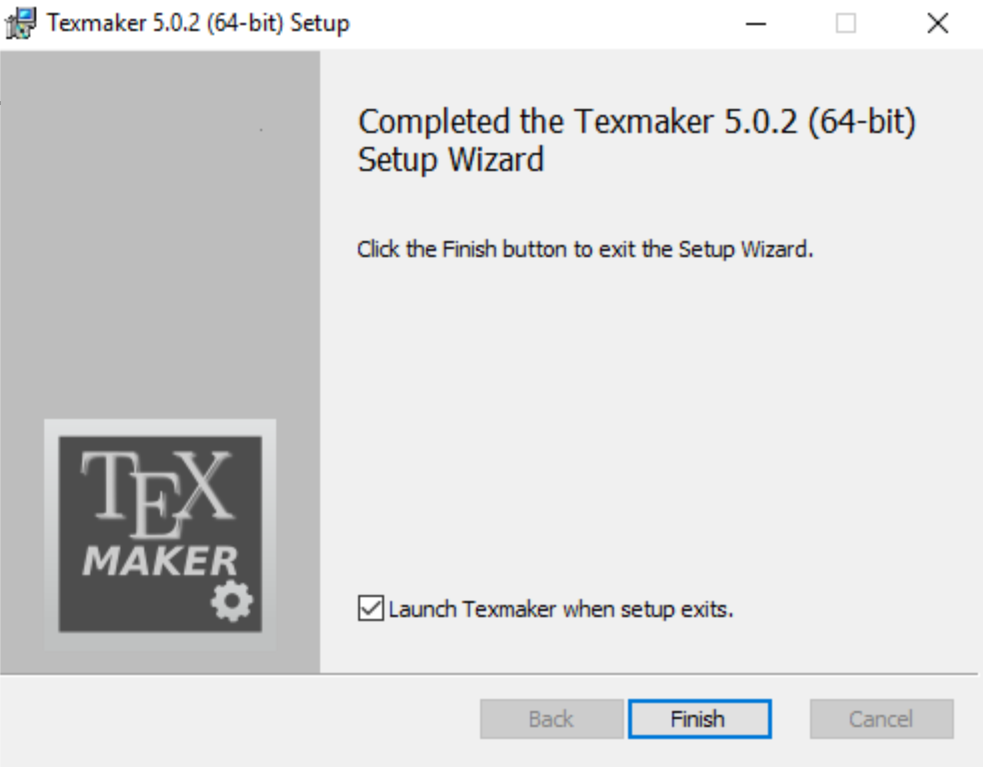
\includegraphics[scale=0.3]{imagens/texmaker/texmaker5.png}
  \end{center}
  \caption{Instalação do TeXMaker - Passo 5.}
  \label{tmk5}
\end{figure}

\subsection{ESTRUTURA DE UM DOCUMENTO LATEX}
O LaTeX funciona a base de comandos que são iniciados com o marcador $\backslash$. Os comandos são escritos nas formas $\backslash$comando ou $\backslash$begin\{comando\}...$\backslash$end\{comando\}. Quando vem escrito nesta última forma, ele é chamado de ambiente. Cada documento começa com $\backslash$begin\{document\} e termina com $\backslash$end\{document\}. Tudo o que vem antes disso é considerado o preâmbulo e tudo o que vem depois de $\backslash$end\{document\} é ignorado.\\
É no preâmbulo que são colocadas todas as informações relacionadas às principais características que terá o documento. O preâmbulo começa com $\backslash$documentclass[opções]\{classe\}.

Opções disponíveis:

•	tamanho da letra. Ex: 10pt, 11pt ou 12pt

•	imprimir em ambos os lados da página ou apenas em um - twoside ou oneside

•	número de colunas - onecolumn ou twocolumn

•	orientação paisagem – landscape

•	tamanho da folha - a4paper, a5paper, letterpaper\\

Classes disponíveis: article, letter, book, report

\newpage
\lstinputlisting[language=TeX,label=lst1,caption={Exemplo de código em LaTeX.}]{codigos/helloworld.tex}

No exemplo da Listagem \ref{lst1}, pode-se observar a estrutura de um documento simples em LaTeX. Para compilar este documento basta ir na barra de ferramentas e clicar na seta ao lado de “Compilar” (Figura \ref{comp}) ou pressionar a tecla F1 no teclado do computador.

\begin{figure}[h!]
  \begin{center}
    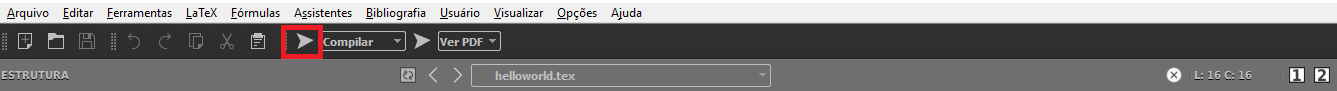
\includegraphics[scale=0.45]{imagens/compilar.png}
  \end{center}
  \caption{Como compilar um documento LaTeX.}
  \label{comp}
\end{figure}

Para facilitar o gerenciamento de documentos grandes, recomenda-se separá-los em um documento principal e uma série de outros sub-documentos. O documento principal e todos os sub-documentos devem estar num mesmo diretório. Os sub-documentos são chamados no documento principal através do comando $\backslash$input nome\_do\_subdocumento. O sumário, as listas de figuras e tabelas são criados no documento principal. Portanto, a estrutura do documento em LaTeX geralmente é constituída de um arquivo fonte salvo em com a extensão .tex contendo um preâmbulo, dos arquivos .tex que compõem documento propriamente dito e da base de dados bibliográficas armazenada num arquivo com a extensão .bib.

Para criar o sumário deve-se utilizar o comando $\backslash$tableofcontents dentro do ambiente document.

Para criar a lista de figuras deve-se utilizar o comando $\backslash$listoffigures dentro do ambiente document.

Para criar a lista de tabelas deve-se utilizar o comando $\backslash$listoftables dentro do ambiente document.

\subsection{PACOTES}
Pacotes são um conjunto de arquivos que implantam uma determinada característica adicional para os documentos escritos em LaTeX. Alguns pacotes já vêm instalados com a distribuição básica do LaTeX, outros podem ser instalados posteriormente de acordo com a necessidade, sendo necessário apenas que o computador esteja conectado à internet. Estes pacotes são inseridos no preâmbulo usando o comando $\backslash$usepackage[opcional]\{pacote\}.

Uma lista de pacotes dispóníveis, junto com manuais e documentações, pode ser encontrada na internet \cite{TeXdoc2018}.

\subsection{SEÇÕES}
Em textos mais longos podem haver varias seções. o LaTeX contém alguns
comandos para dividir o texto deixando-o mais organizado e com estrutura coerente. São eles:

$\backslash$section\{nome\_da\_seção\} - cria uma seção.

$\backslash$subsection\{nome\_da\_subseção\} - cria uma sub-seção.

$\backslash$subsubsection\{nome\_da\_subsubsecção\} - cria uma sub sub-seção.\\

Todas as seções e sub-seções são adicionadas automaticamente ao sumário, com suas respectivas numerações. A Listagem \ref{lst2} mostra um exemplo de como usar seções em um documento LaTeX.

\newpage
\lstinputlisting[language=TeX,label=lst2,caption={Exemplo de como criar seções em LaTeX.}]{codigos/codigosection.tex}

\subsection{INSERINDO FIGURAS}
Para inserir figuras deve-se colocar no preâmbulo o pacote graphicx usando o comando $\backslash$usepackage\{graphicx\} e usar o ambiente figure, conforme a Listagem \ref{lst3}:\\

\lstinputlisting[language=TeX,label=lst3, firstline=7, lastline=10,caption={Como inserir figuras em um documento LaTeX.}]{codigos/codigofigure.tex}

Argumentos de posição:

•	h- A figura ficará onde foi digitado;

•	b- A figura ficará na parte inferior da página;

•	t- A figura ficará na parte superior da página;

•	p- A figura ficará em página separada.\\

A figura deve-se encontrar no mesmo diretório do arquivo fonte .tex, sendo necessário passar o seu nome e extensão como parâmetro de entrada.

Medidas:

•	width (cm) - Define a largura;

•	height (cm) - Define a altura;

•	angle - rotaciona a figura no sentido horário;

•	scale - muda a escala da figura, aumentando ou diminuindo seu tamanho.\\

A Listagem \ref{lst4} apresenta um exemplo do ambiente figure:

\lstinputlisting[language=TeX,label=lst4,caption={Código para inserir a logo do IFTM.}]{codigos/iffigure.tex}

O resultado da Listagem \ref{lst4} é a Figura \ref{if}.\\

\begin{figure}[h]
	\centering
	
\includegraphics[scale=0.4]{imagens/iftm.png}\\
	\caption{Imagem inserida com o código apresentado na Listagem \ref{lst4}.}
	\label{if}
\end{figure}

\subsection{INSERINDO CÓDIGOS FONTE DE LINGUAGEM DE PROGRAMAÇÃO}
Para inserir código no texto deve-se colocar no preâmbulo o pacote listings, usando o comando: $\backslash$usepackage\{listings\}.

Dentro do ambiente document deve-se utilizar o comando:

$\backslash$lstinputlisting[language=linguagem]\{arquivofonte.extensão\}.

Linguagens suportadas: Assembler, C\#, C, Cobol, Delphi, Fortran, HTML, Java, Lua, Pascal, PHP, Prolog, Python, Ruby, SQL, TeX, entre outras.

Utilizando o comando $\backslash$lstset\{\} no preâmbulo, pode-se modificar alguns parâmetros que afetarão a maneira que o código é mostrado no documento, tais como: cor de fundo, tamanho da fonte, adicionar as bordas redor do código, etc.

A Listagem \ref{lst5} mostra um exemplo de inserção de código fonte em um documento LaTeX. O resultado da Listagem \ref{lst5} é a Listagem \ref{lst6}.\\

\lstinputlisting[language=C,label=lst5,caption={Inserção de código fonte no LaTeX.}]{codigos/codigoC.tex}

\newpage
\lstinputlisting[language=C,label=lst6,caption={Código fonte em C inserido utilizando o código da Listagem \ref{lst5}.}]{codigos/helloworldC.c}

\subsection{CRIANDO TABELAS}
Para criar tabelas no LaTeX deve-se utilizar o ambiente table e dentro deste ambiente utilizar o ambiente tabular, pois o ambiente table permite alterar configurações da tabela, como especificar a altura ou largura da tabela e como inserir legenda. Já o ambiente tabular permite construir a tabela em si.

$\backslash$begin\{table\}

$\backslash$begin\{tabular\}[posição]\{especificações\} ... $\backslash$end\{tabular\}

$\backslash$end\{table\}\\

As especificações dizem ao LaTeX o alinhamento a ser usado em cada coluna e as linhas verticais a serem inseridas.\\

\begin{table}[h]
	\centering
	\begin{tabular}{|l|l|}
	\hline
	l & coluna justificada a esquerda \\
	\hline
	c & coluna centralizada \\
	\hline
	r & coluna justificada a direita \\
	\hline
	$|$ & linha vertical \\
	\hline
\end{tabular}\\
\caption{Especificações do ambiente tabular.}
\label{tab1}
\end{table}

Comandos necessários para utilizar tabela:\\

\begin{table}[h]
	\centering
	\begin{tabular}{|l|l|}
	\hline
	\& & separador de colunas \\
	\hline
	$\backslash$ $\backslash$ & inicia uma nova linha \\
	\hline
	$\backslash$hline & linha horizontal \\
	\hline
\end{tabular}
\caption{Comandos para utilizar tabela em LaTeX.}
\label{tab2}
\end{table}

\newpage
A Listagem \ref{lst7} mostra o código utilizado para inserir a tabela \ref{tab2} no documento.\\

\lstinputlisting[language=TeX,label=lst7,firstline=6,lastline=23,caption={Como inserir tabelas em um documento LaTeX.}]{codigos/codigotable.tex}

Existem ferramentas online que facilitam a criação de tabelas \cite{tables2018} .

\subsection{AMBIENTE MATEMÁTICO}
Para inserir fórmulas matemáticas em um documento LaTeX, é necessário criar um ambiente matemático. Existem diversas formas de criar este ambiente sendo elas:

•	\$$\backslash$fórmula\$ - a equação aparece normalmente ao longo do texto

•	$\backslash$($\backslash$fórmula$\backslash$) - a equação aparece normalmente ao longo do texto

•	$\backslash$begin\{math\} $\backslash$fórmula $\backslash$end\{math\} - a equação aparece normalmente ao longo do texto.

•	$\backslash$[ $\backslash$fórmula $\backslash$] - a equação aparece em destaque no centro do texto.

•	$\backslash$begin\{displaymath\} $\backslash$fórmula $\backslash$end\{displaymath\} - a equação aparece em destaque no centro do texto.

•	$\backslash$begin\{equation\} $\backslash$fórmula $\backslash$end\{equation\} - a equação aparece em destaque no centro do texto e numerada.

Para auxiliar na construção de equações, o LaTeX possui uma lista de comandos para exibir símbolos matemáticos que não são acessíveis diretamente pelo teclado, como setas, letras gregas, operadores binários, etc.

A Listagem \ref{lst8} apresenta um exemplo de como inserir uma equação no documento:

\lstinputlisting[language=TeX,label=lst8,caption={Código para inserir a equação da convolução linear.}]{codigos/codigoequation.tex}

O resultado da Listagem \ref{lst8} é a equação \ref{eq:conv}

\begin{equation} \label{eq:conv}
	(f \ast g)(x) = h(x) = \int_{-\infty }^{\infty }f(u)\cdot g(x - u)du 
\end{equation}
 \\
Existem editores online de equações em LaTeX, que permitem construir a equação e fornecem como saída o código em LaTeX para inserir no documento \cite{CodeCogs2018}.

\subsection{INSERINDO REFERÊNCIAS BIBLIOGRÁFICAS}
Para inserir referências no documento LaTeX é necessário criar um documento com o mesmo nome do documento principal e com a extensão .bib, lembrando que ambos devem estar no mesmo diretório. Existe uma sintaxe específica para inserir entradas neste arquivo (Listagem \ref{lst9}):\\

\lstinputlisting[language=TeX,label=lst9,firstline=8,lastline=12,caption={Sintaxe do arquivo .bib.}]{codigos/referenci.tex}

O @tipo refere-se a que tipo de documento está se referenciando, podendo ser:

•	@article para referenciar um artigo de jornal ou revista;

•	@book para referenciar um livro com editora específica;

•	@booklet para referenciar um livro sem editora;

•	@inbook para referenciar um capítulo de um livro, geralmente sem título;

•	@incollection para referenciar um capítulo de um livro com título;

•	@inproceedings para referenciar artigos publicados em anais de conferência;

•	@manual para referenciar documentação técnica;

•	@mastersthesis para referenciar dissertação de mestrado;

•	@misc para uso genérico;

•	@online para referenciar algo dinponível na internet;

•	@phdthesis para referenciar tese de doutorado;

•	@proceedings para referenciar os anais de uma conferência;

•	@techreport para referenciar um relatório publicado por uma instituição.\\

Em alguns tipos existem outros campos de preenchimento não obrigatório. O tipo @book, por exemplo, possui campos como “note” e “isbn” que são opcionais. O “atalho” é usado para se referir à obra ao longo do texto utilizando o comando $\backslash$cite\{atalho\}, portanto, deve ser nomeado com algo que seja intuitivo.

No preâmbulo do documento principal deve-se inserir o pacote abntex2cite utilizando o comando $\backslash$usepackage[alf]\{abntex2cite\}. Este pacote formata as referências no formato da ABNT.

Dentro do ambiente document deve-se inserir os seguintes comandos:

•	$\backslash$newpage - comando para colocar as referências em uma página separada.

•	$\backslash$addcontentsline\{toc\}\{section\}\{Referências\} - comando para adicionar as referências ao sumário.

•	$\backslash$renewcommand\{$\backslash$refname\}\{REFERÊNCIAS\} - comando para mudar o nome da seção caso seja necessário.

•	$\backslash$bibliography\{nome\_do\_arquivo\} - comando para gerar as referências.

Para compilar as referências bibliográficas, deve-se seguir os seguintes passos:

•	Compile o documento principal ao menos uma vez;

•	Compile o arquivo .bib com a opção BibTeX na barra de ferramentas (Figura \ref{compRef}) ou pressionando a tecla F11 no teclado do computador;

\begin{figure}[h]
	\centering
	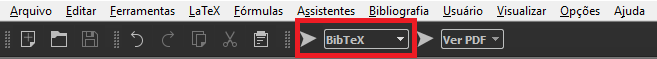
\includegraphics[scale=0.5]{imagens/compilarRef.png}\\
	\caption{Como compilar arquivos de referências bibliográficas.}
	\label{compRef}
\end{figure}

•	Compile o documento principal novamente.

\subsection{CONSIDERAÇÕES SOBRE O CAPÍTULO}
Este capítulo abordou o LaTeX e seus diversos comandos que facilitam a produção de textos com alta qualidade, apresentando um tutorial de como utilizar estes comandos para produzir um documento em LaTeX.